\documentclass{article}
\usepackage[utf8]{inputenc}

\usepackage[toc]{appendix}
\usepackage[margin=2cm]{geometry}
\usepackage{hyperref}
\usepackage{float}
\usepackage[normalem]{ulem}
\useunder{\uline}{\ul}{}
\usepackage{amssymb}
\usepackage{amsmath}
\usepackage{graphicx}
\usepackage{tikz}
\newsavebox{\picbox}
\newcommand{\cutpic}[3]{
  \savebox{\picbox}{\includegraphics[width=#2]{#3}}
  \tikz\node [draw, rounded corners=#1, line width=4pt,
    color=white, minimum width=\wd\picbox,
    minimum height=\ht\picbox, path picture={
      \node at (path picture bounding box.center) {
        \usebox{\picbox}};
    }] {};}


\usepackage{titlesec}

\setcounter{secnumdepth}{4}

\titleformat{\paragraph}
{\normalfont\normalsize\bfseries}{\theparagraph}{1em}{}
\titlespacing*{\paragraph}
{0pt}{3.25ex plus 1ex minus .2ex}{1.5ex plus .2ex}


\def \dueDate{28\textsuperscript{th} May  2023}
\def \ourCompany{Penelope LTD}
\def \ourProduct{Fauna Finder}
\def \weekNumber{34}

\begin{document}
\begin{titlepage}
    \begin{center}
        \null
        \vfill
        
        \cutpic{1cm}{0.4\textwidth}{TitlePage/UpdatedAppIcon.jpg}
        
        \vspace{1cm}
        \Huge
        \textbf{Icarius User Manual}
        
        \vspace{1cm}
        
        \LARGE
        \textbf{Penelope LTD (SwEng Group 2)}\\
        
        \vspace{1cm}
        
        School of PET\\
        
        
        \vspace{1cm}
        
        \dueDate
        
        \vfill
    \end{center}
\end{titlepage}
\tableofcontents
\newpage

\section{Introduction}
Welcome to Icarius, the administrator client used to create, update and delete information on the Fauna Finder database. This user manual will help you through the steps of operating Icarius and is written for administrators who wish to add new birds and edit existing birds for users to view.

\section{System Requirements}
In order to run Icarius, your system will need to meet the following requirements:
\begin{itemize}
    \item Windows Operating System or macOS
    \item At least 100mb of storage space
    \item A network adaptor for constant internet connection
    \item Java SE 8+ or equivalent
\end{itemize}
\section{Application Startup}
\subsubsection{Startup}
Upon startup of the application, the user will be presented with the following screen displaying a prompt for the user to login:
\begin{figure}[h]
    \centering
    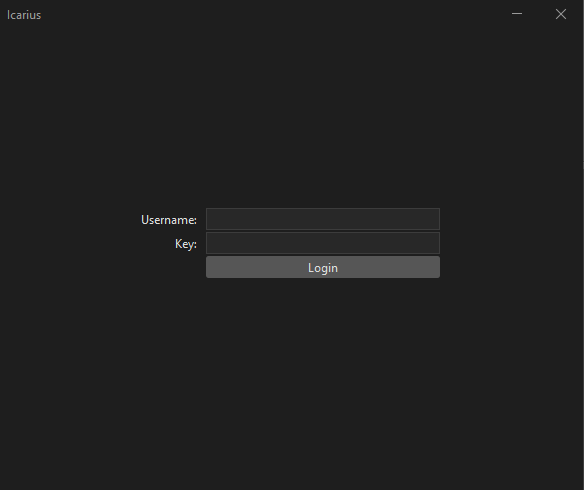
\includegraphics[width=0.6\textwidth]{ApplicationStartup/login.PNG}
\end{figure}

\subsubsection{Logging in}
In order to log in, the user must:
\begin{enumerate}
    \item Enter the username of the admin account in the \textbf{Username} field
    \item Enter the password of the admin account in the \textbf{Key} field
    \item Click the Login button located beneath. \textit{This will then display the \textbf{Administrator View}}
\end{enumerate}
\section{Main Tab}
\subsubsection{Overview}
Upon logging in, the user will be greeted by the \textbf{Main tab}: 
\begin{figure}[h]
    \centering
    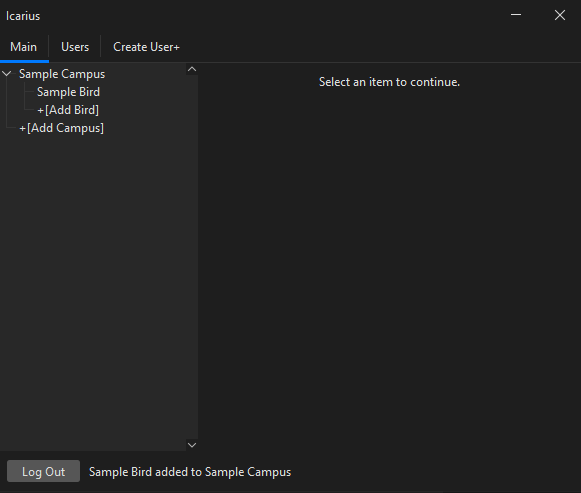
\includegraphics[width=0.6\textwidth]{MainTab/mainTab.PNG}
\end{figure}

The \textbf{Main tab} is where the user can add, edit and remove campuses, and within each campus the user can add, edit and remove birds. The main areas of the \textbf{Main tab} are listed below and are described in the following pages:
\begin{itemize}
    \item Add Campus
    \item View Campus
    \item Edit Campus
    \item Add Bird
    \item View Bird
    \item Edit Bird
    \item Log Out
    \item Confirmation Message
\end{itemize}
The \textbf{Users tab} and \textbf{Create User+ tab} can be accessed by clicking on the respective tab.

\subsubsection{Adding a new campus}
In order to add a new campus, the user must:
\begin{enumerate}
    \item Click on \textbf{+[Add Campus]} located underneath \textbf{Main} on the left. \textit{This will reveal the \textbf{Campus Name} field}
    \begin{figure}[H]
        \centering
        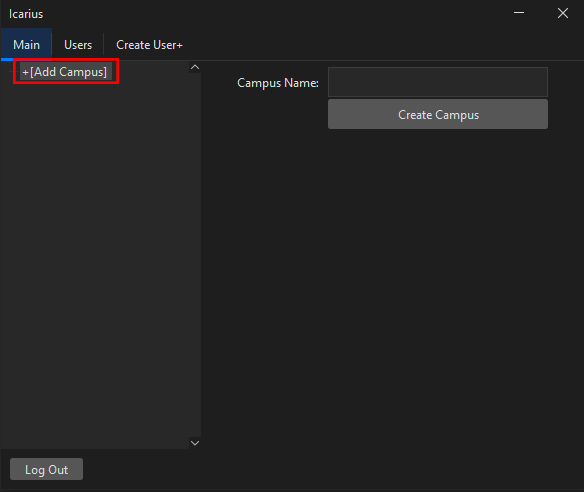
\includegraphics[width=0.6\textwidth]{MainTab/AddCampus/addCampus.PNG}
    \end{figure}
    
    \item Enter the name of the campus in the \textbf{Campus Name} field
    \begin{figure}[H]
        \centering
        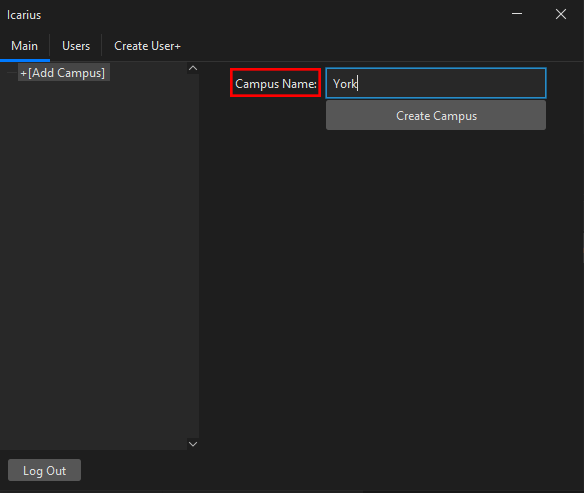
\includegraphics[width=0.6\textwidth]{MainTab/AddCampus/addCampusName.PNG}
    \end{figure}

    \item Click the \textbf{Create Campus} button. \textit{This will add the campus to the database and display a confirmation button alongside the \textbf{Log out} button}
    \begin{figure}[H]
        \centering
        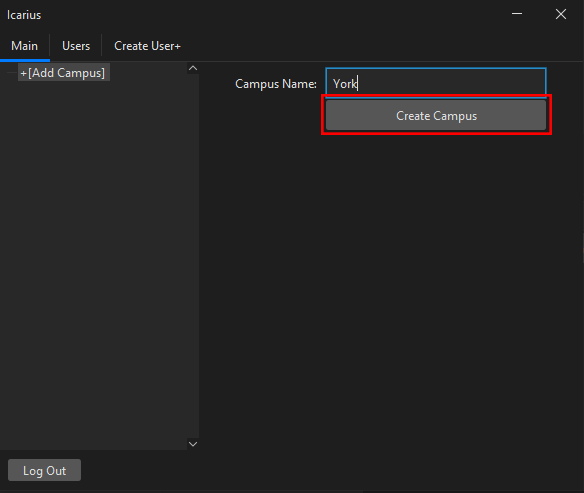
\includegraphics[width=0.6\textwidth]{MainTab/AddCampus/addCampusCreate.PNG}
        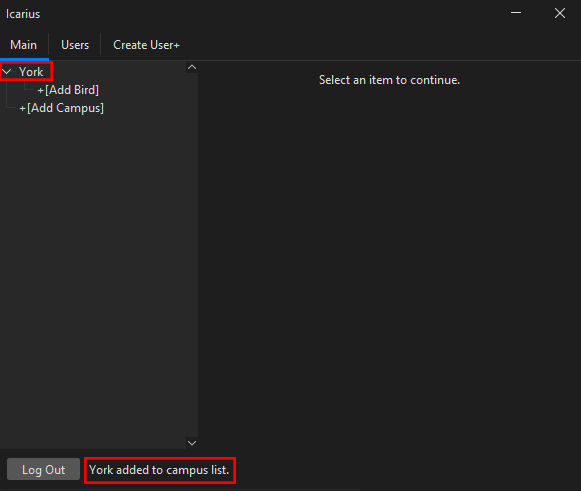
\includegraphics[width=0.6\textwidth]{MainTab/AddCampus/addCampusCreated.PNG}
    \end{figure}
\end{enumerate}

\subsubsection{Editing an existing campus}
In order to edit an existing campus the user must:
\begin{enumerate}
    \item Click on an existing campus. \textit{This will reveal the details of that campus}
    \begin{figure}[H]
        \centering
        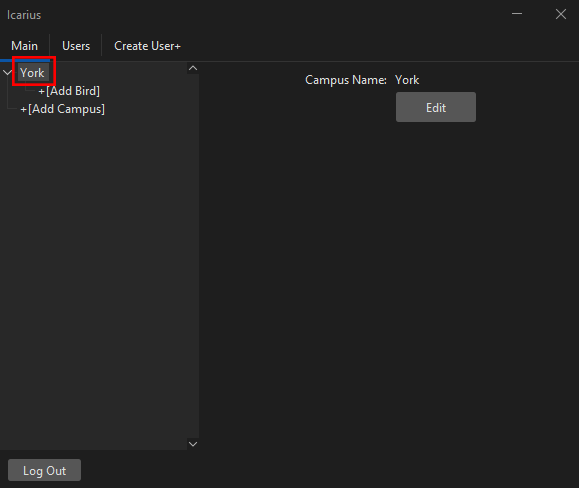
\includegraphics[width=0.6\textwidth]{MainTab/EditCampus/viewCampus.PNG}        
    \end{figure}

    \item Click the \textbf{Edit} button. \textit{This will allow the user to edit the name of the campus alongside the \textbf{Save Changes}, \textbf{Cancel} and \textbf{Delete} buttons } 
    \begin{figure}[H]
        \centering
        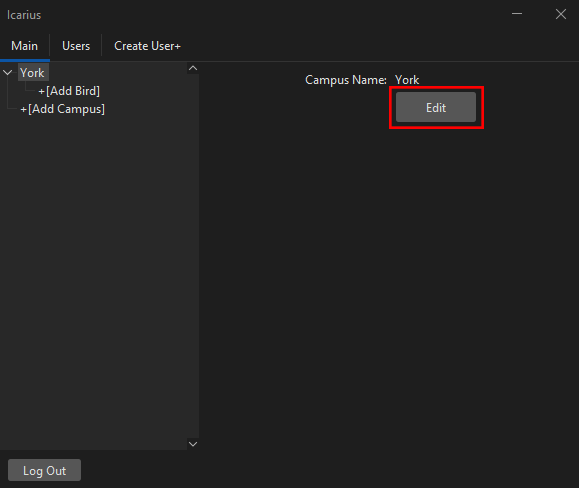
\includegraphics[width=0.6\textwidth]{MainTab/EditCampus/editCampus.PNG}
        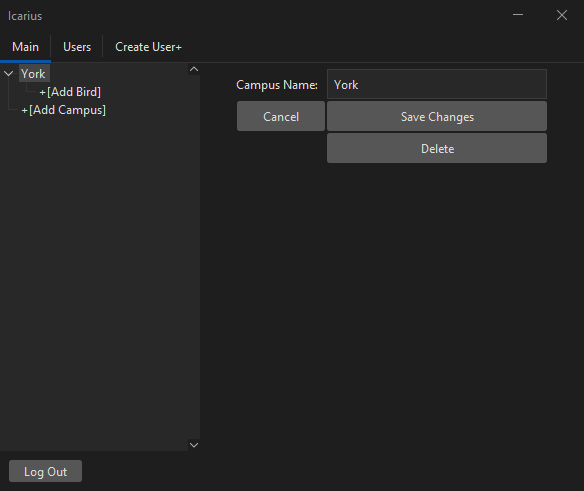
\includegraphics[width=0.6\textwidth]{MainTab/EditCampus/editCampusView.PNG}
    \end{figure}

    \item Clicking the \textbf{Save Changes} button will save the edits made to the campus to the database, whilst clicking the \textbf{Cancel} button cancels those edits made. The \textbf{Delete} button can be clicked to remove the campus from the database. \textit{Choosing \textbf{Save Changes} or \textbf{Delete} displays a confirmation button alongside the \textbf{Log out} button}

    \textbf{Save Changes:}
    \begin{figure}[H]
        \centering
        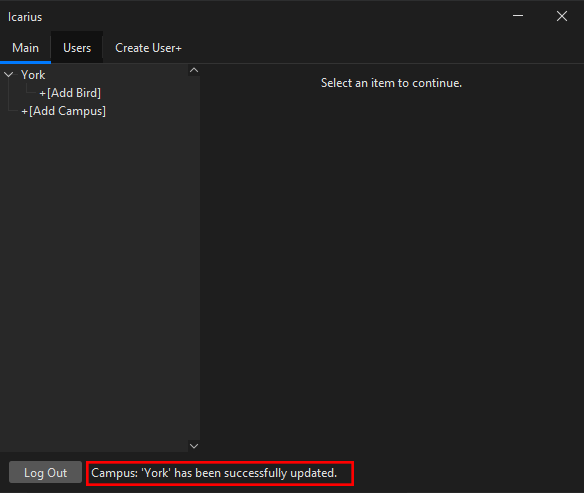
\includegraphics[width=0.6\textwidth]{MainTab/EditCampus/editCampusSave.PNG}
    \end{figure}

    \textbf{Delete:}
    \begin{figure}[H]
        \centering
        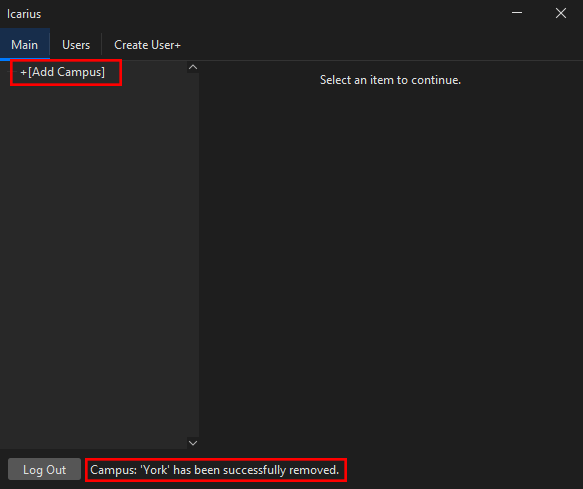
\includegraphics[width=0.6\textwidth]{MainTab/EditCampus/editCampusDelete.PNG}
    \end{figure}
\end{enumerate}

\subsubsection{Adding a new bird to a campus}
In order to add a new bird to a campus, the user must:
\begin{enumerate}
    \item Click on \textbf{+[Add Bird]} located underneath the selected campus. \textit{This will reveal the \textbf{Bird Name} field}
    \begin{figure}[H]
        \centering
        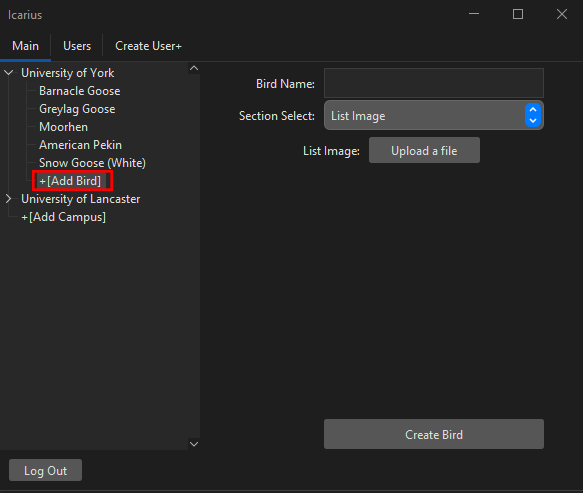
\includegraphics[width=0.6\textwidth]{MainTab/AddBird/addBird.PNG}
    \end{figure}
    
    \item Enter the name of the bird in the \textbf{Bird Name} field
    \begin{figure}[H]
        \centering
        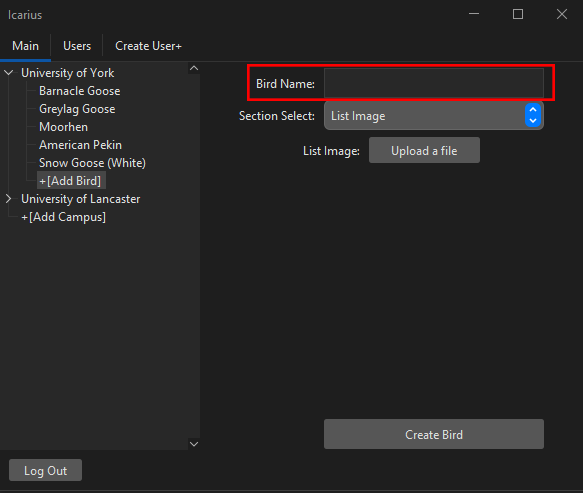
\includegraphics[width=0.6\textwidth]{MainTab/AddBird/addBirdName.PNG}
    \end{figure}

    \item Click the \textbf{Section Select} drop-down list to view each attribute of the bird
    \begin{figure}[H]
        \centering
        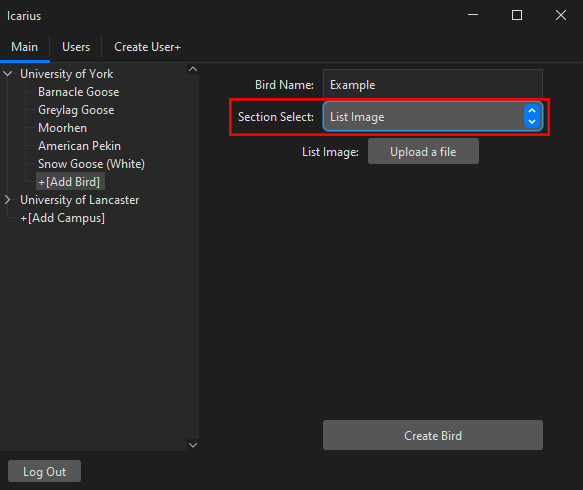
\includegraphics[width=0.6\textwidth]{MainTab/AddBird/addBirdSelect.PNG}
        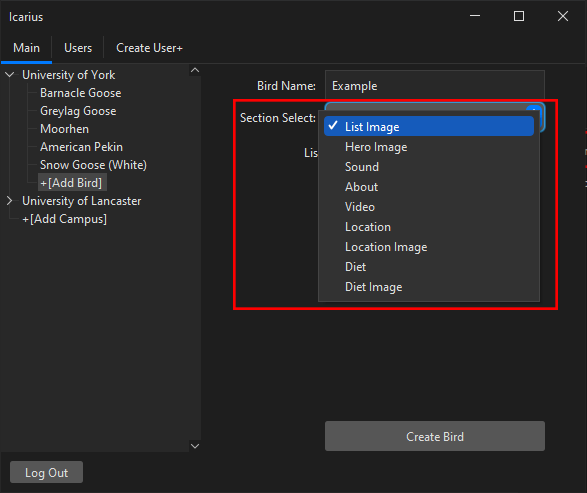
\includegraphics[width=0.6\textwidth]{MainTab/AddBird/addBirdDropdown.PNG}
    \end{figure}
    The attributes of a bird are as follows:
    \begin{itemize}
        \item \textbf{List Image:} The image of the bird as it appears in the bird list in FaunaFinder
        \item \textbf{Hero Image:} The image of the bird once clicked on in FaunaFinder
        \item \textbf{Sound:} The audio soundbite of the bird
        \item \textbf{About:} The information about the bird
        \item \textbf{Video:} The video footage of the bird
        \item \textbf{Location:} The location of the bird
        \item \textbf{Location Image:} The image of the location of the bird
        \item \textbf{Diet:} The information about the diet of the bird
        \item \textbf{Diet Image:} The image of the diet of the bird
    \end{itemize}
    
    \item Click on each section to fill in each attribute of the bird. \textit{Each attribute must be complete before the creation of the bird can occur}
    \begin{itemize}
        \item \textbf{List Image, Hero Image, Location Image and Diet Image:}
        An image can be uploaded for the attributes that require it by clicking on \textbf{Upload a file}. \textit{This will display the image underneath to confirm the correct image has been uploaded}
        \begin{figure}[H]
            \centering
            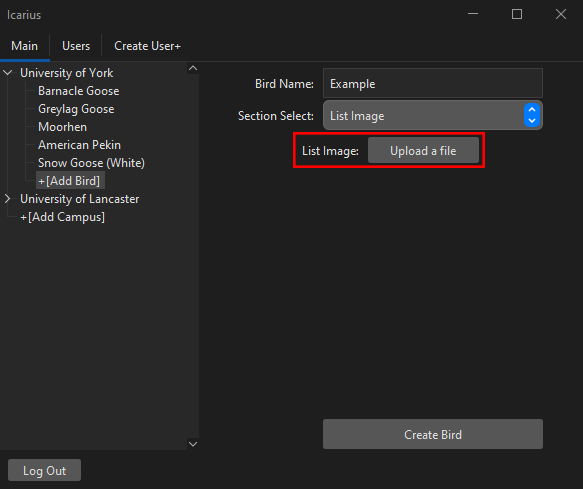
\includegraphics[width=0.6\textwidth]{MainTab/AddBird/addBirdImage.PNG}
            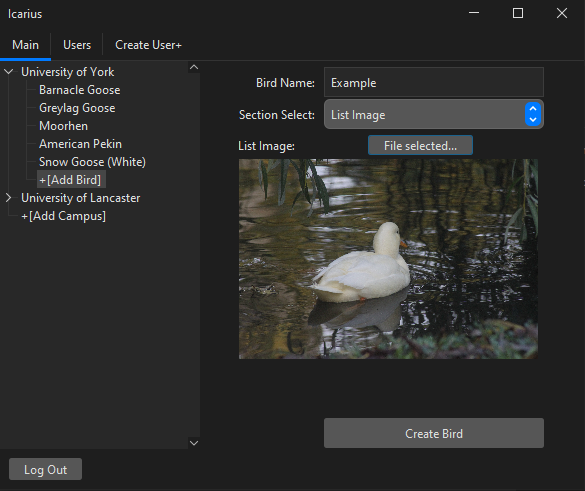
\includegraphics[width=0.6\textwidth]{MainTab/AddBird/addBirdImageSelected.PNG}
        \end{figure}
        
        \item \textbf{About, Location and Diet:}
        Information can be input for the attributes that require it by typing in the text area
        \begin{figure}[H]
            \centering
            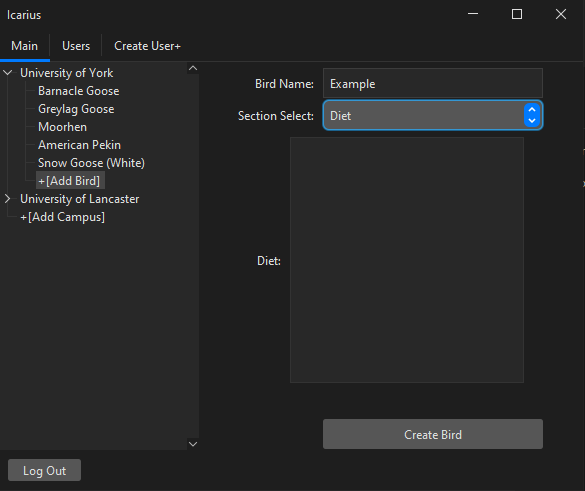
\includegraphics[width=0.6\textwidth]{MainTab/AddBird/addBirdText.PNG}
        \end{figure}

        \item \textbf{Sound:}
        An audio file can be uploaded by clicking on clicking on \textbf{Upload a file}. The audio can be sampled by clicking on \textbf{Play audio}
        \begin{figure}[H]
            \centering
            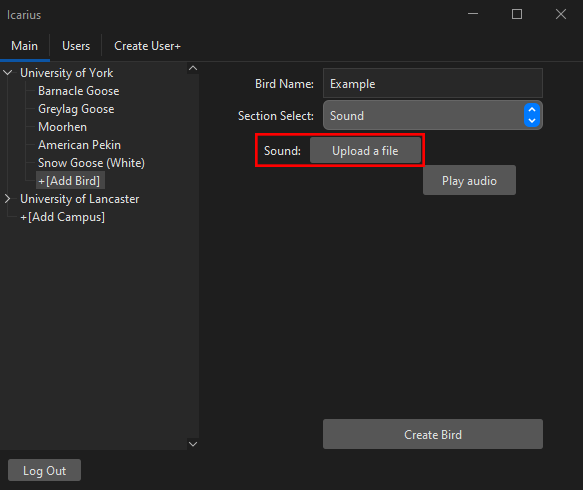
\includegraphics[width=0.6\textwidth]{MainTab/AddBird/addBirdAudio.PNG}
            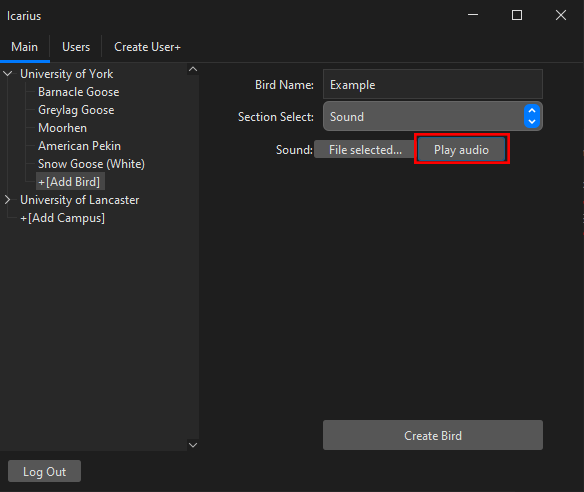
\includegraphics[width=0.6\textwidth]{MainTab/AddBird/addBirdAudioSelected.PNG}
        \end{figure}

        \item \textbf{Video:}
        A video file can be uploaded by clicking on clicking on \textbf{Upload a file}. A thumbnail preview of the video will be displayed below
        \begin{figure}[H]
            \centering
            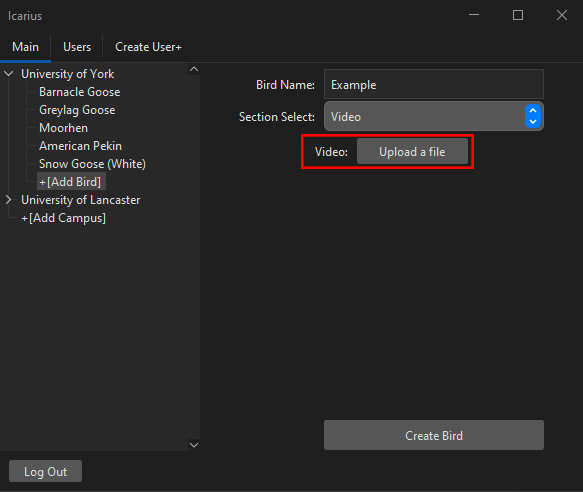
\includegraphics[width=0.6\textwidth]{MainTab/AddBird/addBirdVideo.PNG}
            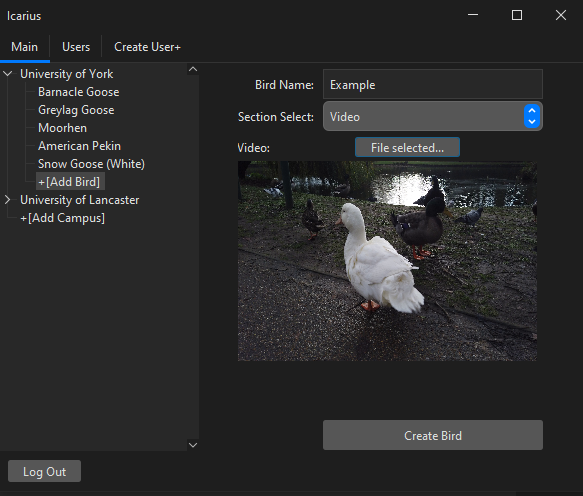
\includegraphics[width=0.6\textwidth]{MainTab/AddBird/addBirdVideoSelected.PNG}
        \end{figure}
    \end{itemize}
    
    \item Click the \textbf{Create Bird} button. \textit{This will add the bird to the database and display a confirmation button alongside the \textbf{Log out} button}
    \begin{figure}[H]
        \centering
        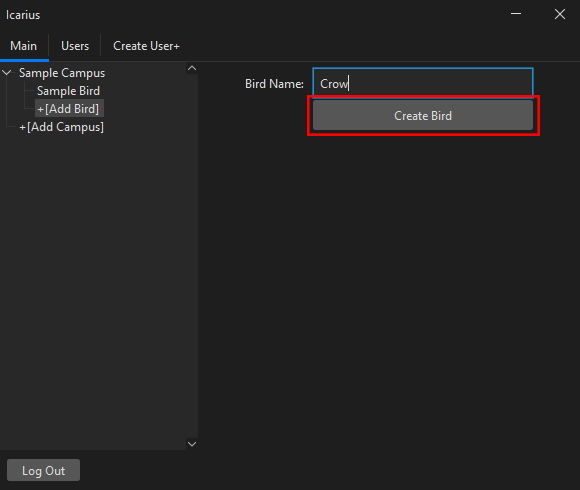
\includegraphics[width=0.6\textwidth]{MainTab/AddBird/addBirdCreate.PNG}
        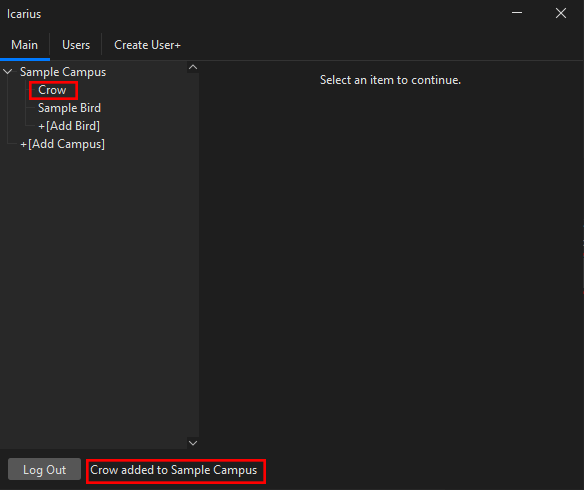
\includegraphics[width=0.6\textwidth]{MainTab/AddBird/addBirdCreated.PNG}
    \end{figure}
\end{enumerate}

\subsubsection{Editing an existing bird}
In order to edit an existing bird the user must:
\begin{enumerate}
    \item Click on an existing bird underneath the selected campus. \textit{This will reveal the details of that bird}
    \begin{figure}[H]
        \centering
        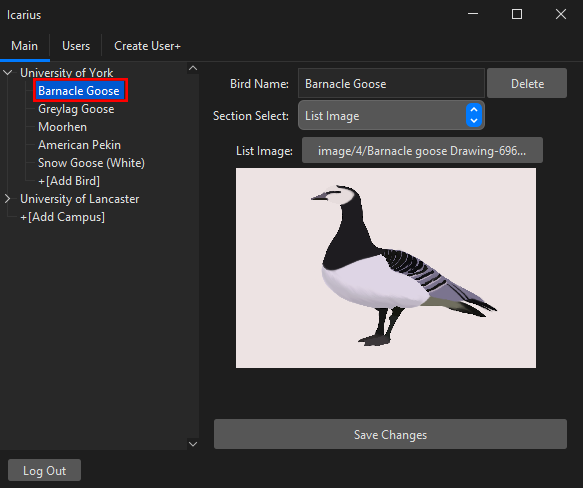
\includegraphics[width=0.6\textwidth]{MainTab/EditBird/editBirdView.PNG}
    \end{figure}

    \item From here, each of the attributes of the bird can be edited by selecting them from the \textbf{Section Select} drop-down list
    \begin{figure}[H]
        \centering
        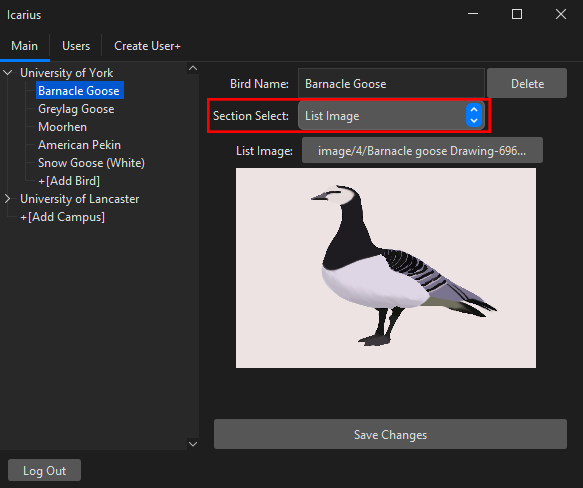
\includegraphics[width=0.6\textwidth]{MainTab/EditBird/editBirdSection.PNG}
    \end{figure}

    \item Clicking the \textbf{Save Changes} button will save the edits made to the bird to the database, whilst clicking the \textbf{Cancel} button cancels those edits made. The \textbf{Delete} button can be clicked to remove the bird from the database. \textit{Choosing \textbf{Save Changes} or \textbf{Delete} displays a confirmation button alongside the \textbf{Log out} button}

    \textbf{Save Changes:}
    \begin{figure}[H]
        \centering
        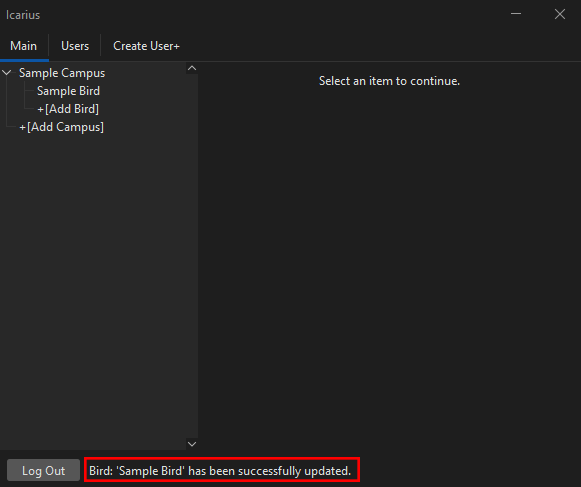
\includegraphics[width=0.6\textwidth]{MainTab/EditBird/saveChanges.PNG}
    \end{figure}

    \textbf{Delete:}
    \begin{figure}[H]
        \centering
        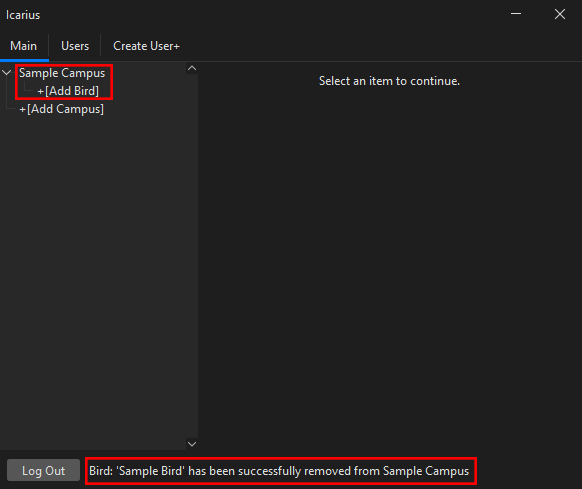
\includegraphics[width=0.6\textwidth]{MainTab/EditBird/deleteBird.PNG}
    \end{figure}
    

    
\end{enumerate}

\section{Users Tab}
\subsubsection{Overview}
The \textbf{Users tab} allows the user to view and edit existing user's information and allocate them to particular campuses. 

\begin{figure}[H]
    \centering
    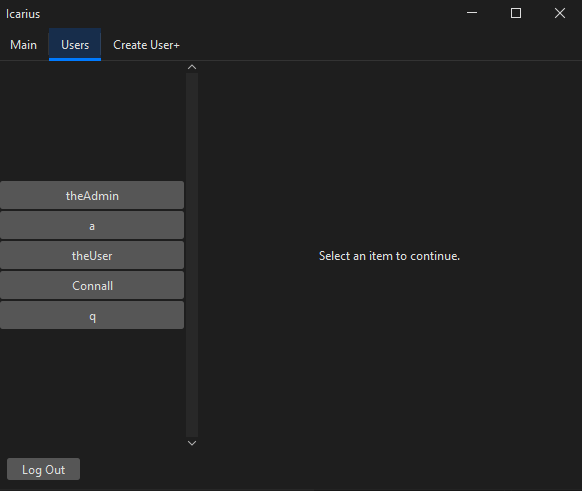
\includegraphics[width=0.6\textwidth]{UsersTab/usersTabOverview.PNG}
\end{figure}

\subsubsection{Viewing an existing user}
In order to view an existing user, the user must:
\begin{enumerate}
    \item Click on a user located in the left panel of the tab. \textit{This will reveal the attributes of that user on the right}
    \begin{figure}[H]
        \centering
        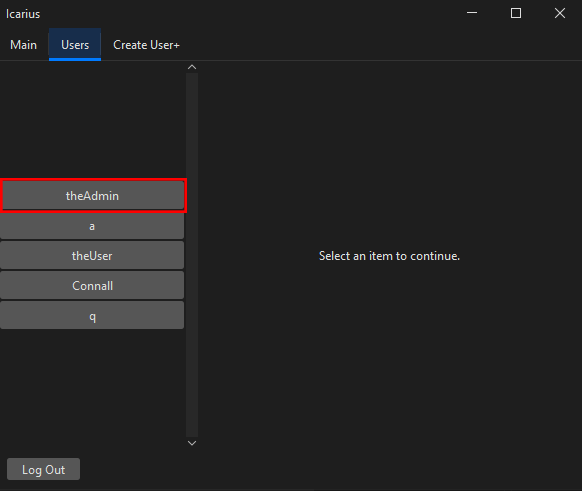
\includegraphics[width=0.6\textwidth]{UsersTab/viewUser/viewUser.png}
        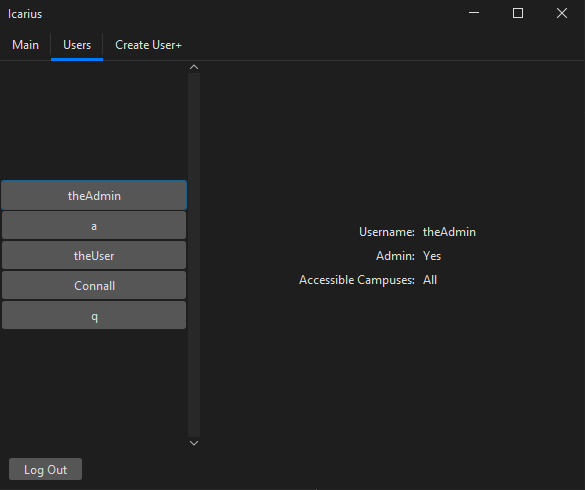
\includegraphics[width=0.6\textwidth]{UsersTab/viewUser/viewUserSelected.png}
    \end{figure}
    The attributes of a user are as follows:
    \begin{itemize}
        \item \textbf{Username:} The selected users username
        \item \textbf{Admin:} Displays whether the user is an admin or not
        \item \textbf{Accessible Campuses:} A list of all of the campuses the user is able to make edits to within the main tab. If the selected user is an admin this will just say \textbf{All}
    \end{itemize}
\end{enumerate}

\subsubsection{Editing an existing user}
Admin users cannot have their attributes be changed.

In order to edit an existing user, the user must:
\begin{enumerate}
    \item Click on a user located in the left panel of the tab.  \textit{This will reveal the attributes of that user on the right}
    \begin{figure}[H]
        \centering
        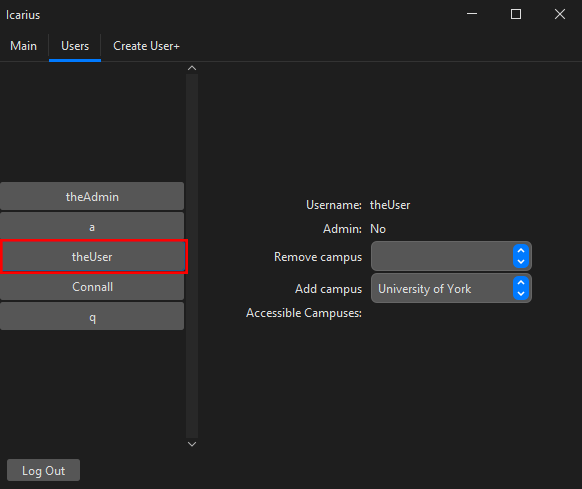
\includegraphics[width=0.6\textwidth]{UsersTab/editUser/editUser.png}
    \end{figure}

    \item A campus can be added to the user by clicking on the \textbf{Add Campus} drop-down list. \textit{This will reveal each campus in the database}
    \begin{figure}[H]
        \centering
        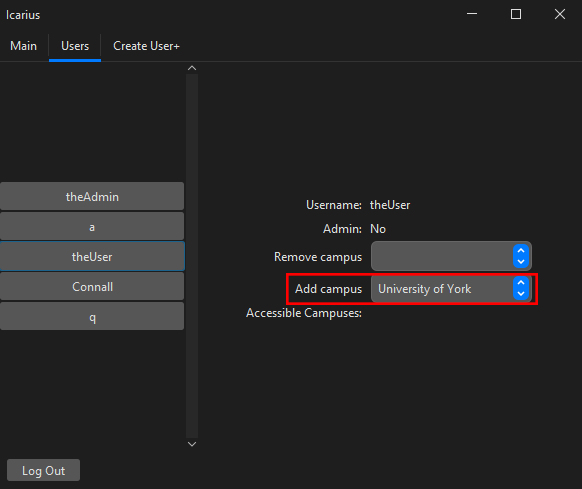
\includegraphics[width=0.6\textwidth]{UsersTab/editUser/editUserAdd.png}
        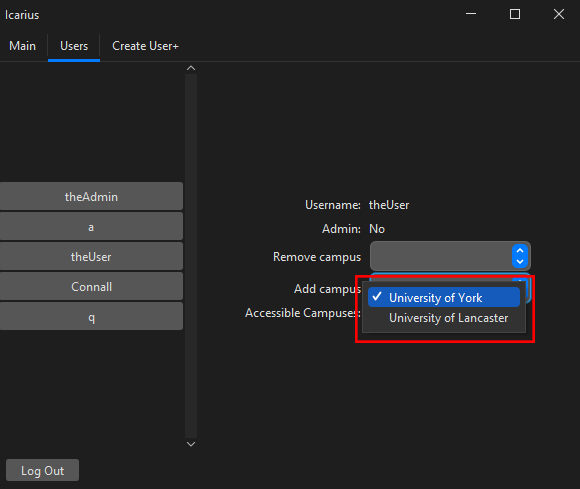
\includegraphics[width=0.6\textwidth]{UsersTab/editUser/editUserAddView.png}
    \end{figure}
    
    Similarly, a campus can be removed from the user by clicking on the \textbf{Remove Campus} drop-down list.
    \begin{figure}[H]
        \centering
        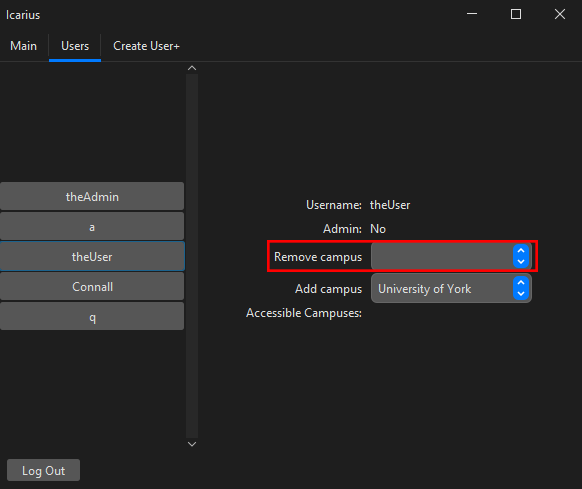
\includegraphics[width=0.6\textwidth]{UsersTab/editUser/editUserRemove.png}
        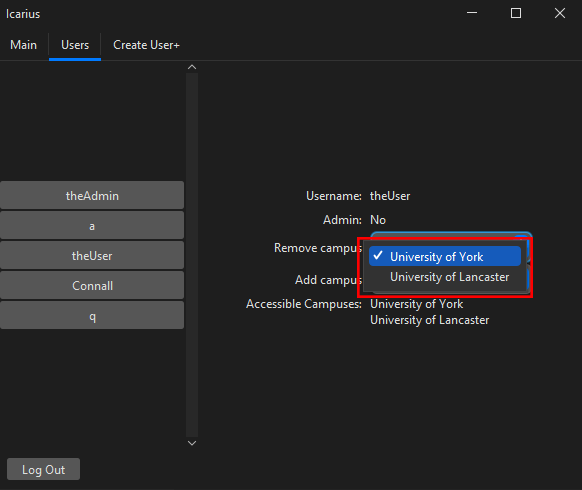
\includegraphics[width=0.6\textwidth]{UsersTab/editUser/editUserRemoveView.png}
    \end{figure}
\end{enumerate}
\section{Create User Tab}
\subsubsection{Overview}
The \textbf{Create User tab} Allows for the creation of a new user in the server, setting their username, password and role, either being an admin or a user.

\begin{figure}[H]
    \centering
    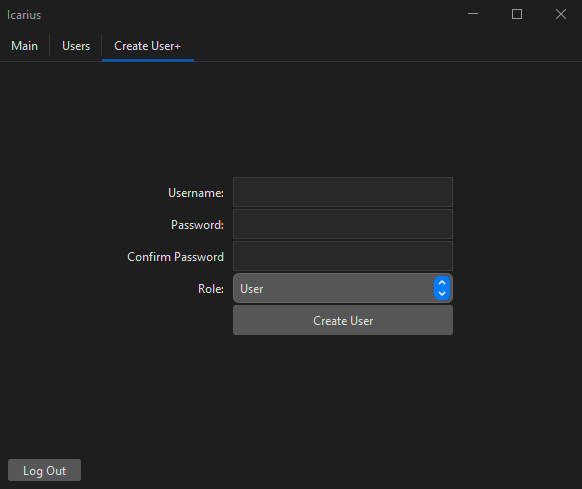
\includegraphics[width=0.6\textwidth]{CreateUserTab/createUserOverview.PNG}
\end{figure}

\subsubsection{Creating a new user}
In order to add a new user, the user must:
\begin{enumerate}
    \item Fill the \textbf{Username}, \textbf{Password} and \textbf{Confirm Password} fields
    \begin{figure}[H]
        \centering
        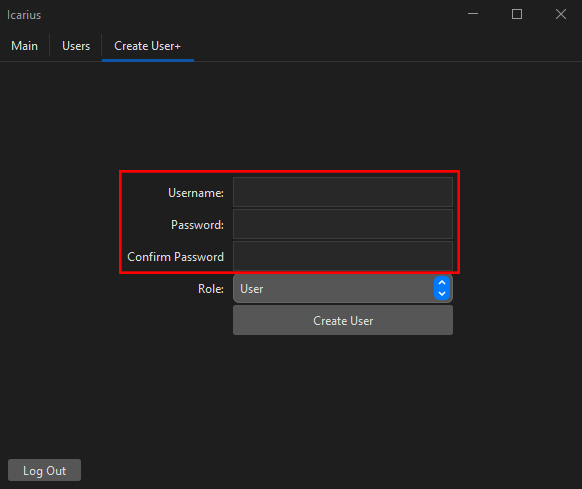
\includegraphics[width=0.6\textwidth]{CreateUserTab/CreateUser/createUserText.PNG}
    \end{figure}

    \item Click on the \textbf{Role} drop-down list to select the new user’s role. This will be either an admin or a user
    \begin{figure}[H]
        \centering
        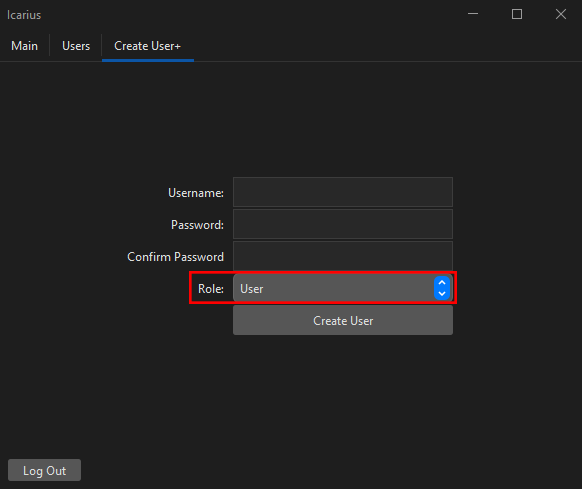
\includegraphics[width=0.6\textwidth]{CreateUserTab/CreateUser/createUserRole.PNG}
        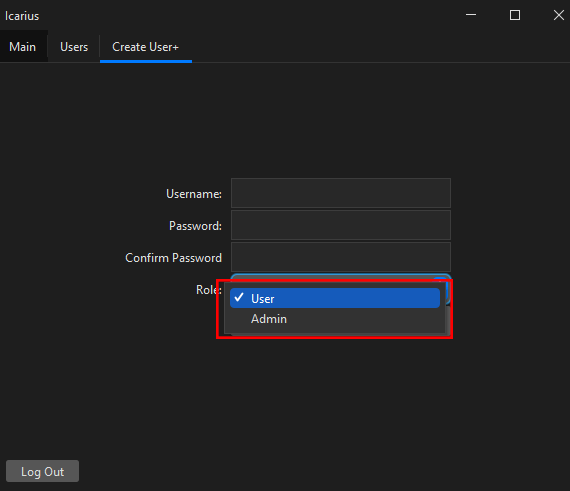
\includegraphics[width=0.6\textwidth]{CreateUserTab/CreateUser/createUserRoleView.PNG}
    \end{figure}

    \item Click on \textbf{Create User}. \textit{This will add the user to the database}
    \begin{figure}[H]
        \centering
        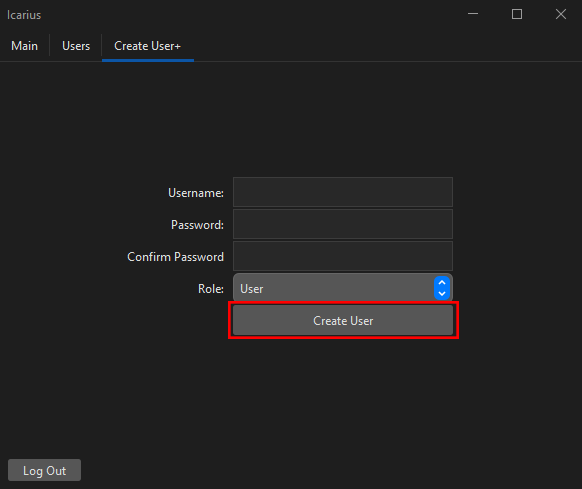
\includegraphics[width=0.6\textwidth]{CreateUserTab/CreateUser/createUserCreate.PNG}
    \end{figure}
\end{enumerate}
\section{Conclusion}
Thank you for making it through the Icarius user manual. We hope that it has guided you through the features of the application, as well as how to use them.

\bibliographystyle{IEEEtran}
\bibliography{bibtex.bib}
\end{document}